\chapter{Ensayos y resultados experimentales}

\section{Introducción}

Una vez implementado el sistema de control diseñado en la placa de desarrollo Nexys 3, se realizan una serie de ensayos para verificar su correcto funcionamiento. Estos ensayos fueron realizados en forma progresiva, en un principio probando sólamente el generador PWM junto con el ADC en un esquema lazo abierto. Luego de ir confirmando el correcto funcionamiento, se fueron agregando más componentes para finalmente realizar un ensayo con el lazo cerrado de tensión.

\section{Pruebas a lazo abierto}

Las primeras pruebas realizadas a lazo abierto consistieron en la utilización del controlador PWM para las señales de los transistores del convertidor CC-CC. Luego, se implementó al controlador del conversor analógico-digital para permitir la variación del ciclo de trabajo mediante un potenciómetro, cuyo valor era filtrado por el filtro diseñado e implementado a \SI{1.5}{\kilo\hertz}.

\section{Pruebas a lazo cerrado}

\subsection{Lazo de control de corriente}

El primer ensayo a lazo cerrado consistió en el control de la corriente por el inductor del convertidor CC-CC. En este sistema fueron utilizados los componentes ya probados anteriormente: el controlador PWM; el controlador del ADC; y el filtro de corriente de \SI{1.5}{\kilo\hertz}. Para poder cerrar el lazo, se incorporaron dos nuevos elementos: la referencia, para poder establecer un valor en el cual la corriente se establezca; y el controlador PI, para poder calcular la acción de control que permita seguir a la referencia.

\begin{figure}[hbt!]
  \centering
  \subfloat[Escalón negativo de \SI{3}{\ampere}.]{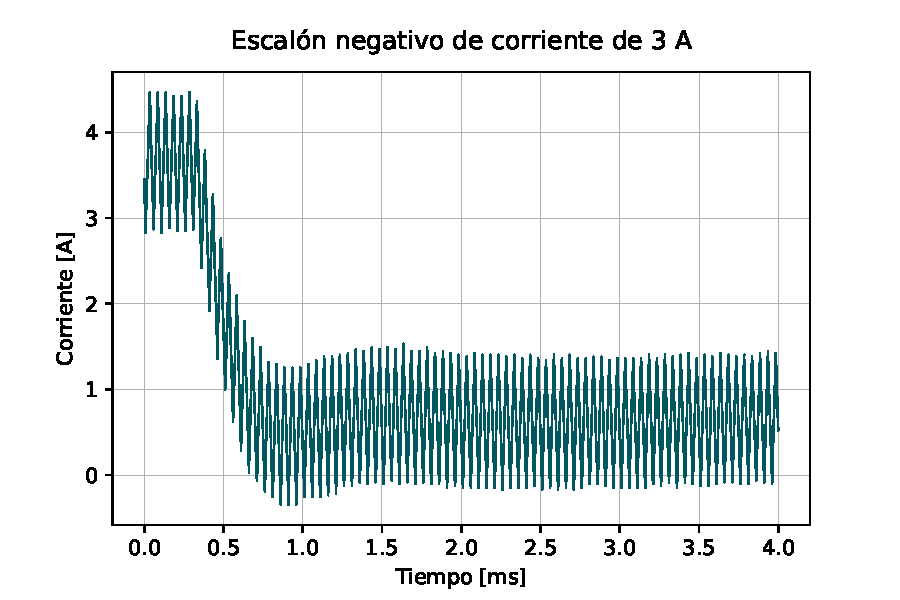
\includegraphics[width=0.45\textwidth]{Imágenes/Ensayos/Lazo interno de corriente/Fuente de potencia/Escalón negativo de corriente.pdf}}    
  \subfloat[Escalón positivo de \SI{3}{\ampere}.]{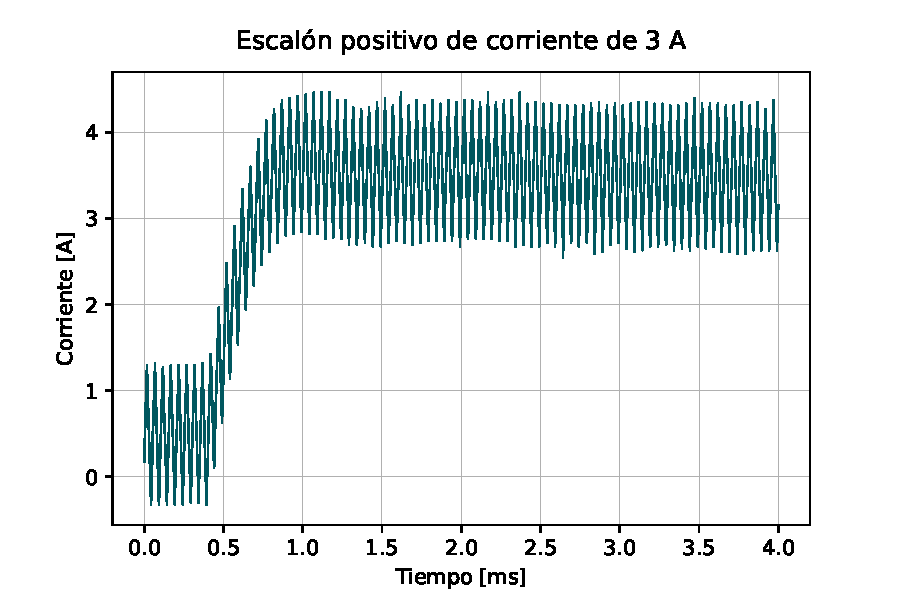
\includegraphics[width=0.45\textwidth]{Imágenes/Ensayos/Lazo interno de corriente/Fuente de potencia/Escalón positivo de corriente.pdf}}
  \caption{Resultados de los ensayos del lazo de corriente.}
  \label{escalones-lazo-corriente}
\end{figure}

Como medida de seguridad, se implementaron llaves que permiten habilitar o deshabilitar el integrador del controlador. Además, este componente posee una saturación a su salida, para evitar el cálculo de un ciclo de trabajo mayor a 1 o 100\%; y el método anti-windup explicado anteriormente.

Realizando escalones de \SI{3}{\ampere} con este sistema de control, se obtuvieron los siguientes resultados de la Figura \ref{escalones-lazo-corriente}. Se puede observar que la corriente se establece en el nuevo valor de referencia en cuestión de microsegundos sin causar un sobrepico abrupto o peligroo, y por lo tanto se considera que el lazo de corriente controla satisfactoramiente a la variable de estado.

\subsection{Lazo de control de tensión}

Para el lazo de control de tensión se realizaron una serie de ensayos bajo distintas condiciones para determinar la performance del sistema de control implementado. Los primeros ensayos consistieron en pequeños escalones en la tensión de referencia. Una vez verificado el correcto funcionamiento del sistema a lazo cerrado, se realizaron pruebas más demandantes al lazo de control, variando la resistencia de carga y observando la respuesta de la corriente de entrada y tensión de salida. En la Figura \ref{var-r-lazo-tension} pueden observarse las respuestas de ambas variables de estado para un salto de \SI{20}{\ohm} a \SI{40}{\ohm}.

En ambos casos puede observarse una rápida y robusta recuperación del nivel de tensión establecido por la referencia. Para el caso del escalón positivo de resistencia, existe una leve oscilación que termina en el establecimiento de la tensión de salida en un valor de \SI{24}{\volt}.

\begin{figure}[hbt!]
  \centering
  \subfloat[Escalón negativo de \SI{40}{\ohm} a \SI{20}{\ohm}.]{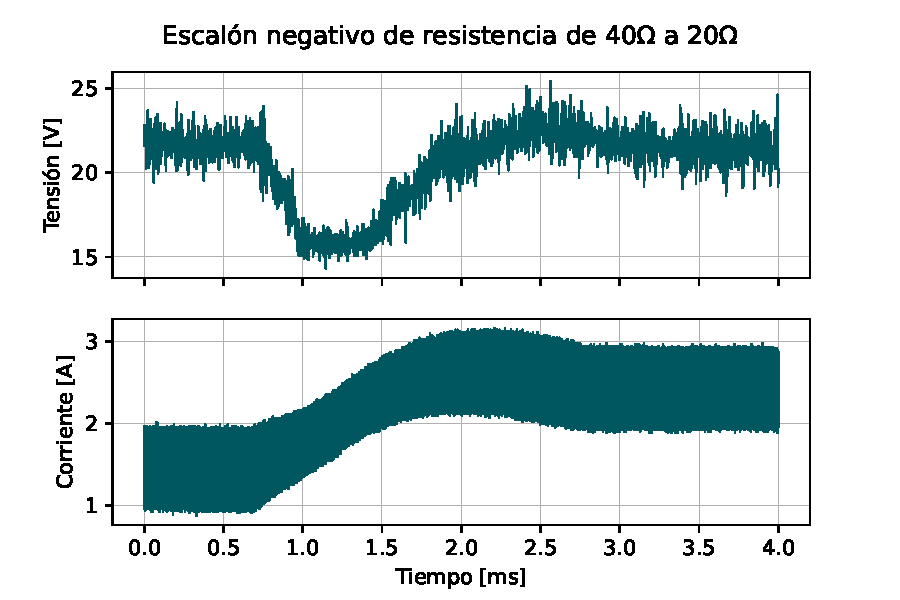
\includegraphics[width=0.45\textwidth]{Imágenes/Ensayos/Lazo externo de tensión/Escalón negativo de resistencia.pdf}}    
  \subfloat[Escalón positivo de \SI{20}{\ohm} a \SI{40}{\ohm}.]{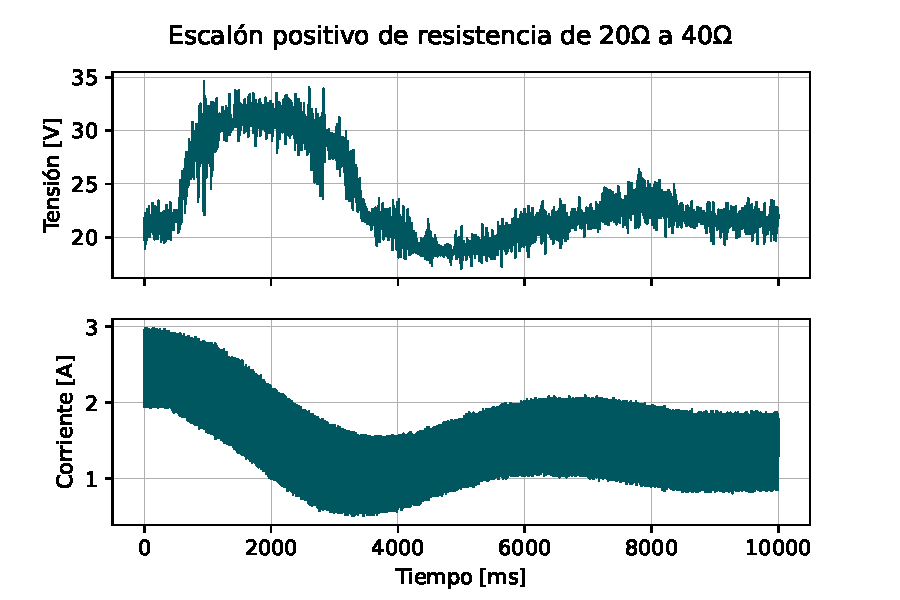
\includegraphics[width=0.45\textwidth]{Imágenes/Ensayos/Lazo externo de tensión/Escalón positivo de resistencia.pdf}}
  \caption{Resultados de los ensayos del lazo de tensión.}
  \label{var-r-lazo-tension}
\end{figure}

\newpage